\section{ROLLO Verification}
To verify \gls{ROLLO}'s optimization capabilities, I conducted multiple verification 
studies: commonly used evolutionary algorithm single and multi objective benchmark problems
and a nuclear reactor-specific problem. 
Together, they prove that \gls{ROLLO}'s evolutionary algorithm is correctly implemented 
and suitable for conducting nuclear reactor optimization problems. 

\subsection{Ackley Function}
The Ackley function is a non-convex function, commonly used as a performance test 
for single-objective optimization algorithms \cite{ackley_connectionist_2012}: 
\begin{align}
    f(x) &= -a \cdot exp \left(-b\sqrt{\frac{1}{d}\Sigma_{i=1}^dx_i^2}\right) - 
    exp \left(\frac{1}{d}\Sigma_{i=1}^d cos(cx_i)\right) + a + exp(1) 
\end{align}
The recommended variable values are $a=20$, $b=0.2$, and $c=2\pi$
\cite{sfu_ackley_nodate}. 
The Ackley function's global optimum point is $f(0,0) = 0$. 
Figure \ref{fig:ackley} shows the resulting two-variable Ackley function.
\begin{figure}[H]
    \centering
    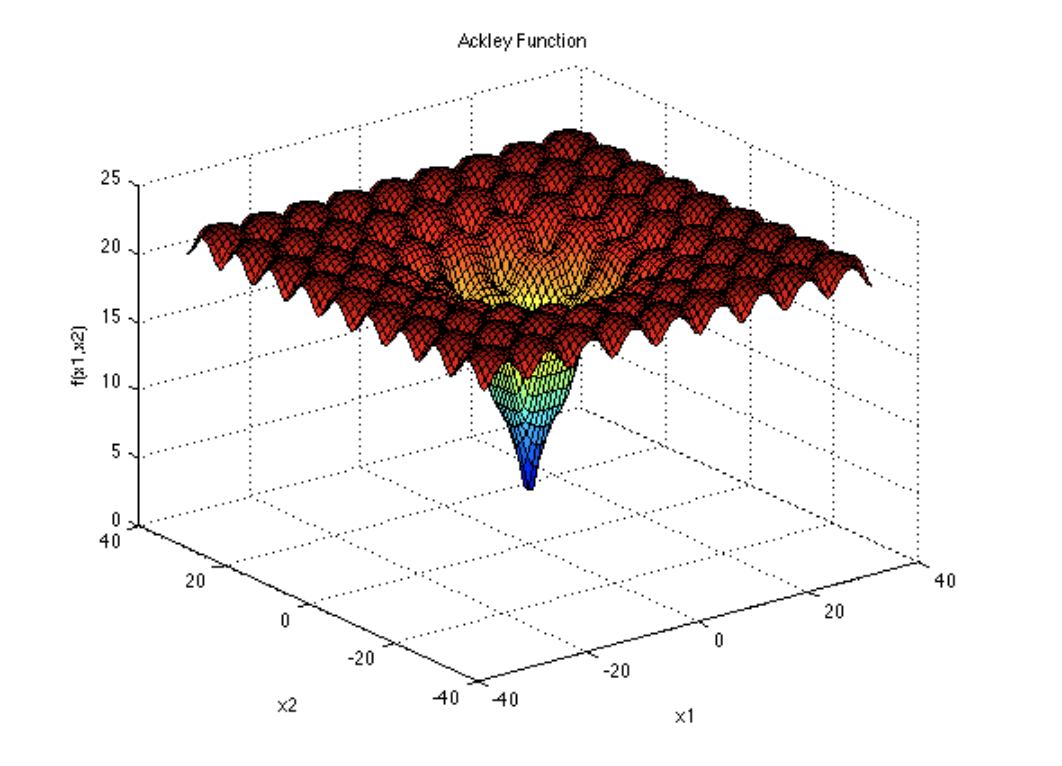
\includegraphics[width=0.65\linewidth]{figures/ackley.png} 
    \caption{Two variable Ackley function \cite{sfu_ackley_nodate}.}
    \label{fig:ackley}
\end{figure}
 
I added an integration test to \gls{ROLLO} that checks that a default \gls{ROLLO} 
simulation will find the Ackley function's global optimum point. 
If \gls{ROLLO} performed sub-optimally, it would return one of the Ackley 
function's many local minimums. 
\gls{ROLLO} successfully finds the global optimum point, and thus passes the 
integration test. 

\subsection{Binh and Korn Function}
The Binh and Korn function 

\subsection{Pu-239 Critical Bare Sphere}
To ensure \gls{ROLLO} works correctly while coupled with OpenMC, I run \gls{ROLLO} 
to find the critical radius for a $^{239}Pu$ bare sphere. 
The solution to this problem is well studied and available \cite{blanchard_updated_1999}. 
Blanchard et al reported that with MCNP4b code and ENDF/B-VI data library, the 
critical mass of a Pu239 bare sphere is 10.00 kg which corresponds to a diameter 
of 9.9cm \cite{blanchard_updated_1999}.
Figure \ref{fig:verification-sphere} shows the ROLLO input file for this verification 
problem. 
In the input file, I vary the radius between 1.0 and 8.0cm, with the objective of 
minimizing radius, while constraining the problem to have $k_{eff} >= 1.0$.
\begin{figure}[H]
    \begin{minted}[
        frame=lines,
        framesep=2mm,
        baselinestretch=1.2,
        fontsize=\footnotesize,
        linenos
        ]{json}
        {"control_variables": {
                "radius": {"min": 1.0, "max": 8.0}},
            "evaluators": {
                "openmc": {
                    "input_script": "critical_sphere.py",
                    "inputs": ["radius"],
                    "outputs": ["keff", "radius"],
                    "keep_files": false}},
            "constraints": {"keff": {"operator": [">="], "constrained_val": [1.0]}},
            "algorithm": {
                "parallel": "multiprocessing",
                "objective": ["min"],
                "optimized_variable": ["radius"]
            }}
    \end{minted}
    \caption{\acrfull{ROLLO} JSON input file for finding the minimum radius for 
    a $^{239}Pu$ Critical Bare Sphere.}
    \label{fig:verification-sphere}
\end{figure}
\pagebreak
Figure \ref{fig:critical_sphere.py} shows the OpenMC template used in the 
\gls{ROLLO} simulation. 
\begin{figure}[H]
    \begin{minted}[
        frame=lines,
        framesep=2mm,
        baselinestretch=1.2,
        fontsize=\footnotesize,
        linenos
        ]{python}
            import openmc 
            import numpy as np

            pu = openmc.Material()
            pu.set_density("g/cm3", 19.84)
            pu.add_nuclide("Pu239", 1)
            mats = openmc.Materials([pu])
            
            radius = {{radius}}
            
            fuel_sphere = openmc.Sphere(r=radius, boundary_type='vacuum')
            fuel_cell = openmc.Cell(fill=pu, region=-fuel_sphere)
            univ = openmc.Universe(cells=[fuel_cell])
            geom = openmc.Geometry(univ)
            
            settings = openmc.Settings()
            settings.batches = 100
            settings.inactive = 20
            settings.particles = 20000
            settings.temperature = {"multipole": True, "method": "interpolation"}
            
            mats.export_to_xml()
            geom.export_to_xml()
            settings.export_to_xml()
            openmc.run()
    \end{minted}
    \caption{OpenMC template input file used in ROLLO simulation to find the 
    minimum radius for a $^{239}Pu$ Critical Bare Sphere.}
    \label{fig:critical_sphere.py}
\end{figure}  

\gls{ROLLO} successfully finds the critical radius of the $^{239}Pu$ bare sphere 
to be 4.9856cm which corresponds to approximately a 9.9cm diameter. 
The critical sphere's $k_{eff}$ value is 1.00919 $\pm$ 0.00048. 
Figure \ref{fig:verification-radius} and \ref{fig:verification-keff} show the 
radius and $k_{eff}$ evolution through the evolutionary algorithm's 
generations. 
They demonstrate how the average radius and $k_{eff}$ converge
towards the critical radius while keeping $k_{eff} > 1$ with improvements from 
each generation.
\begin{figure}[]
    \centering
    \begin{subfigure}{\textwidth}
    \makebox[\textwidth][c]{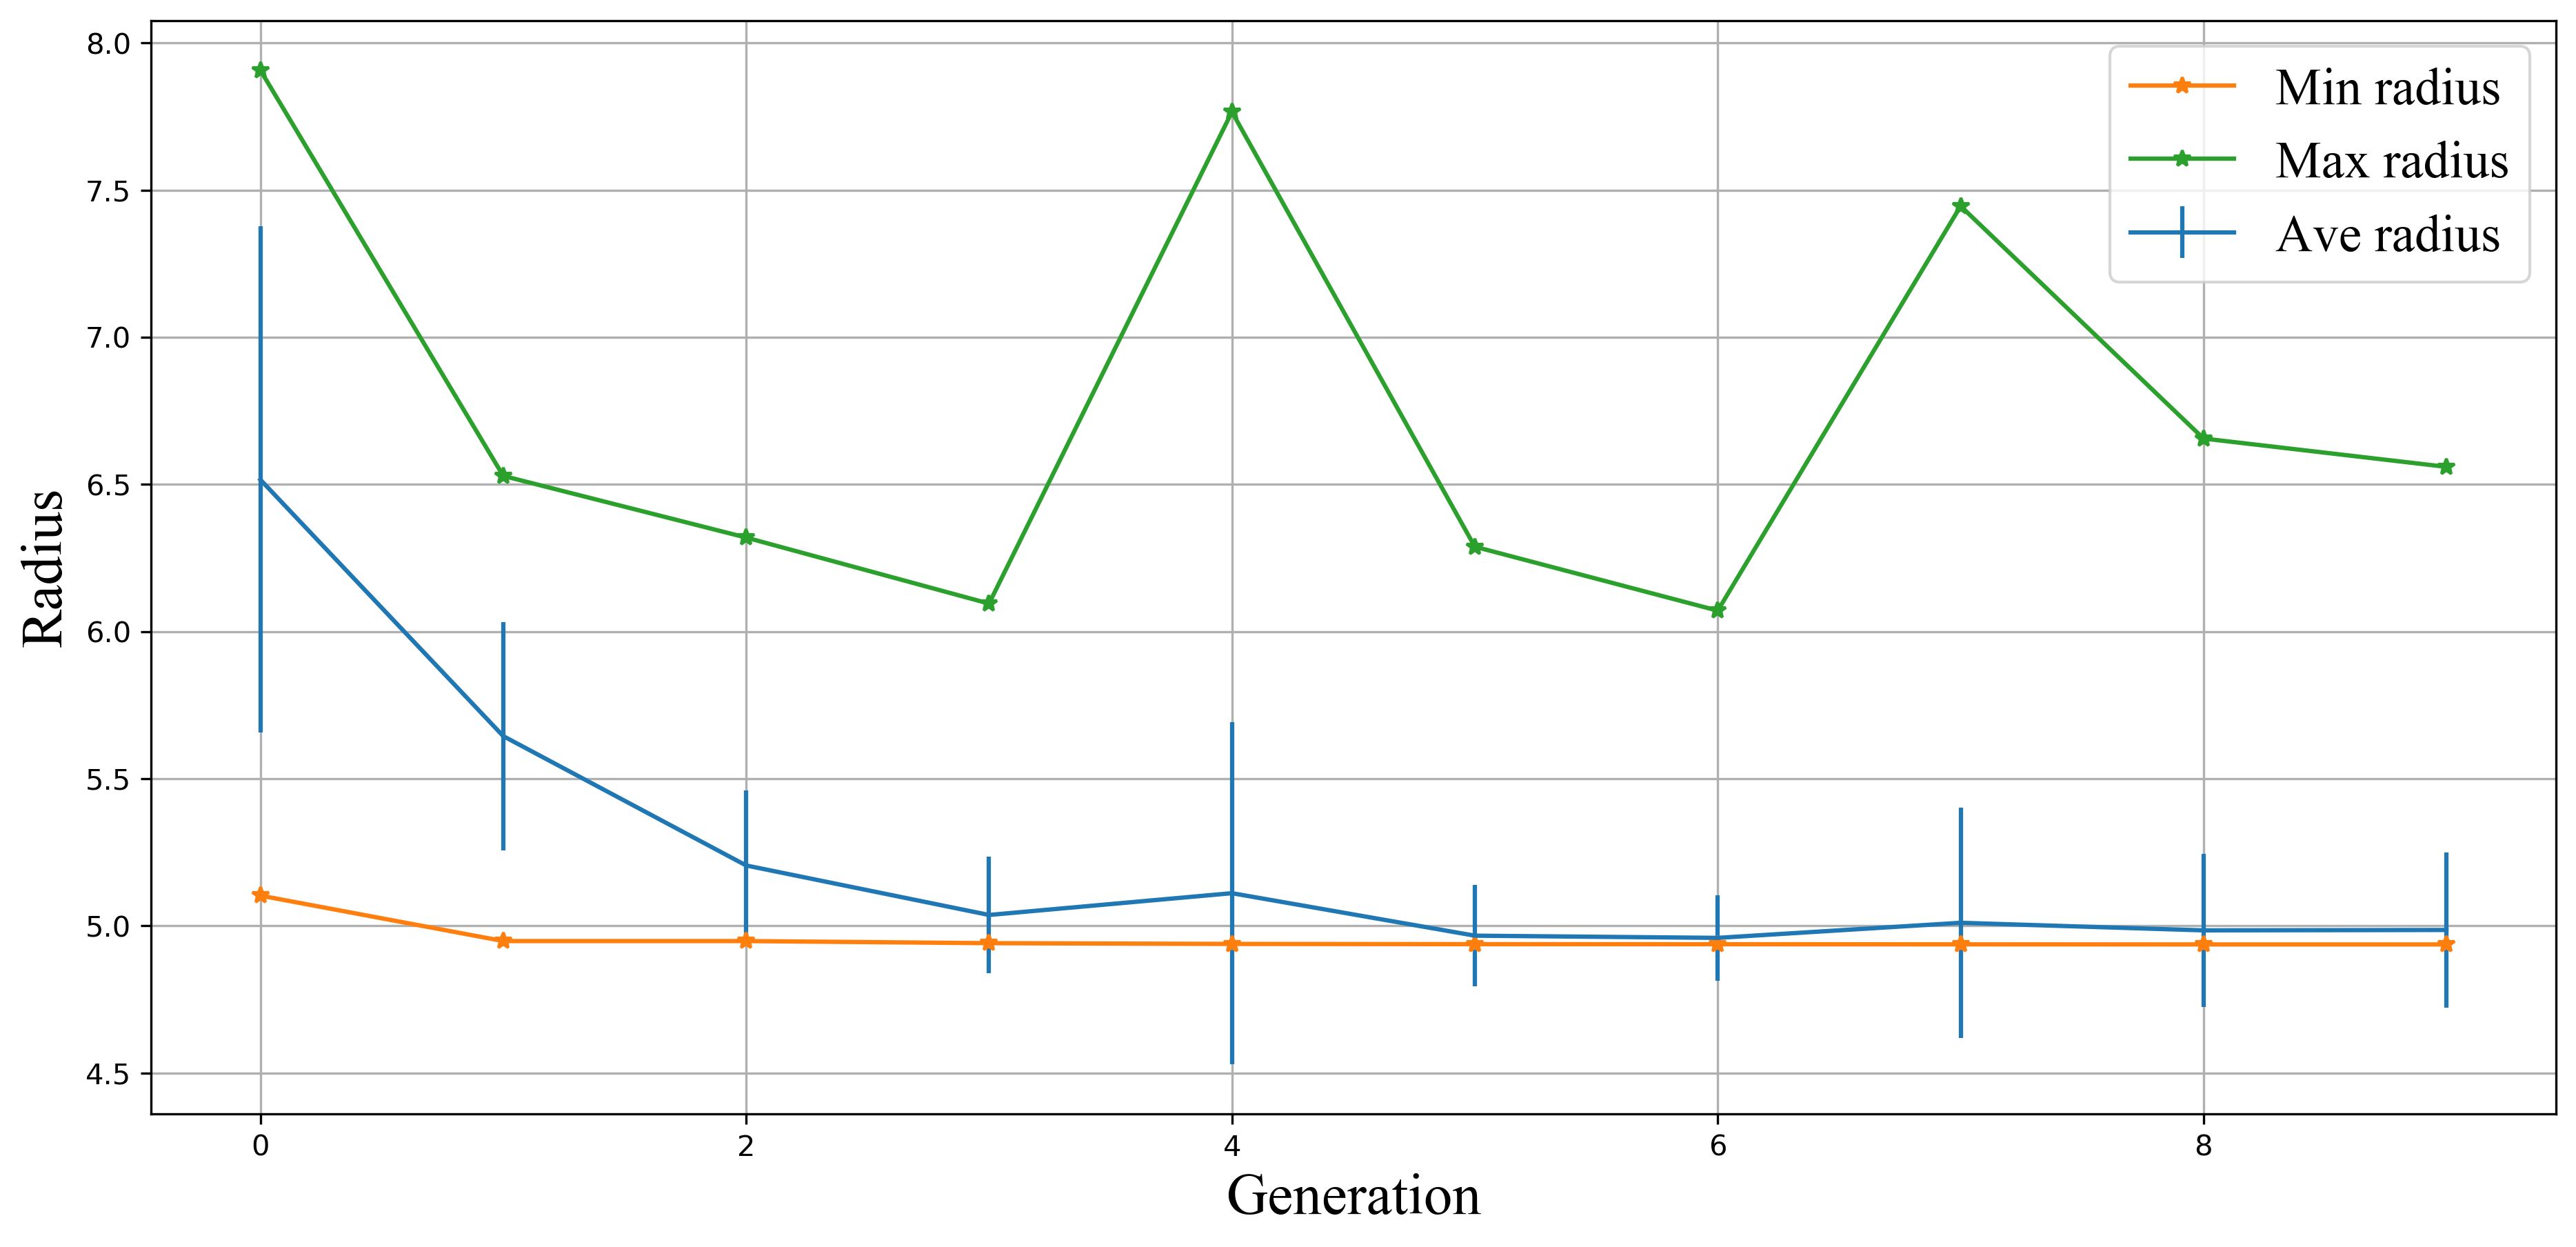
\includegraphics[width=1.1\linewidth]{verification-radius.png}} 
    \caption{Minimum, average, and maximum radius values evolution.}
    \label{fig:verification-radius}
    \end{subfigure}
    \begin{subfigure}{\textwidth}
        \makebox[\textwidth][c]{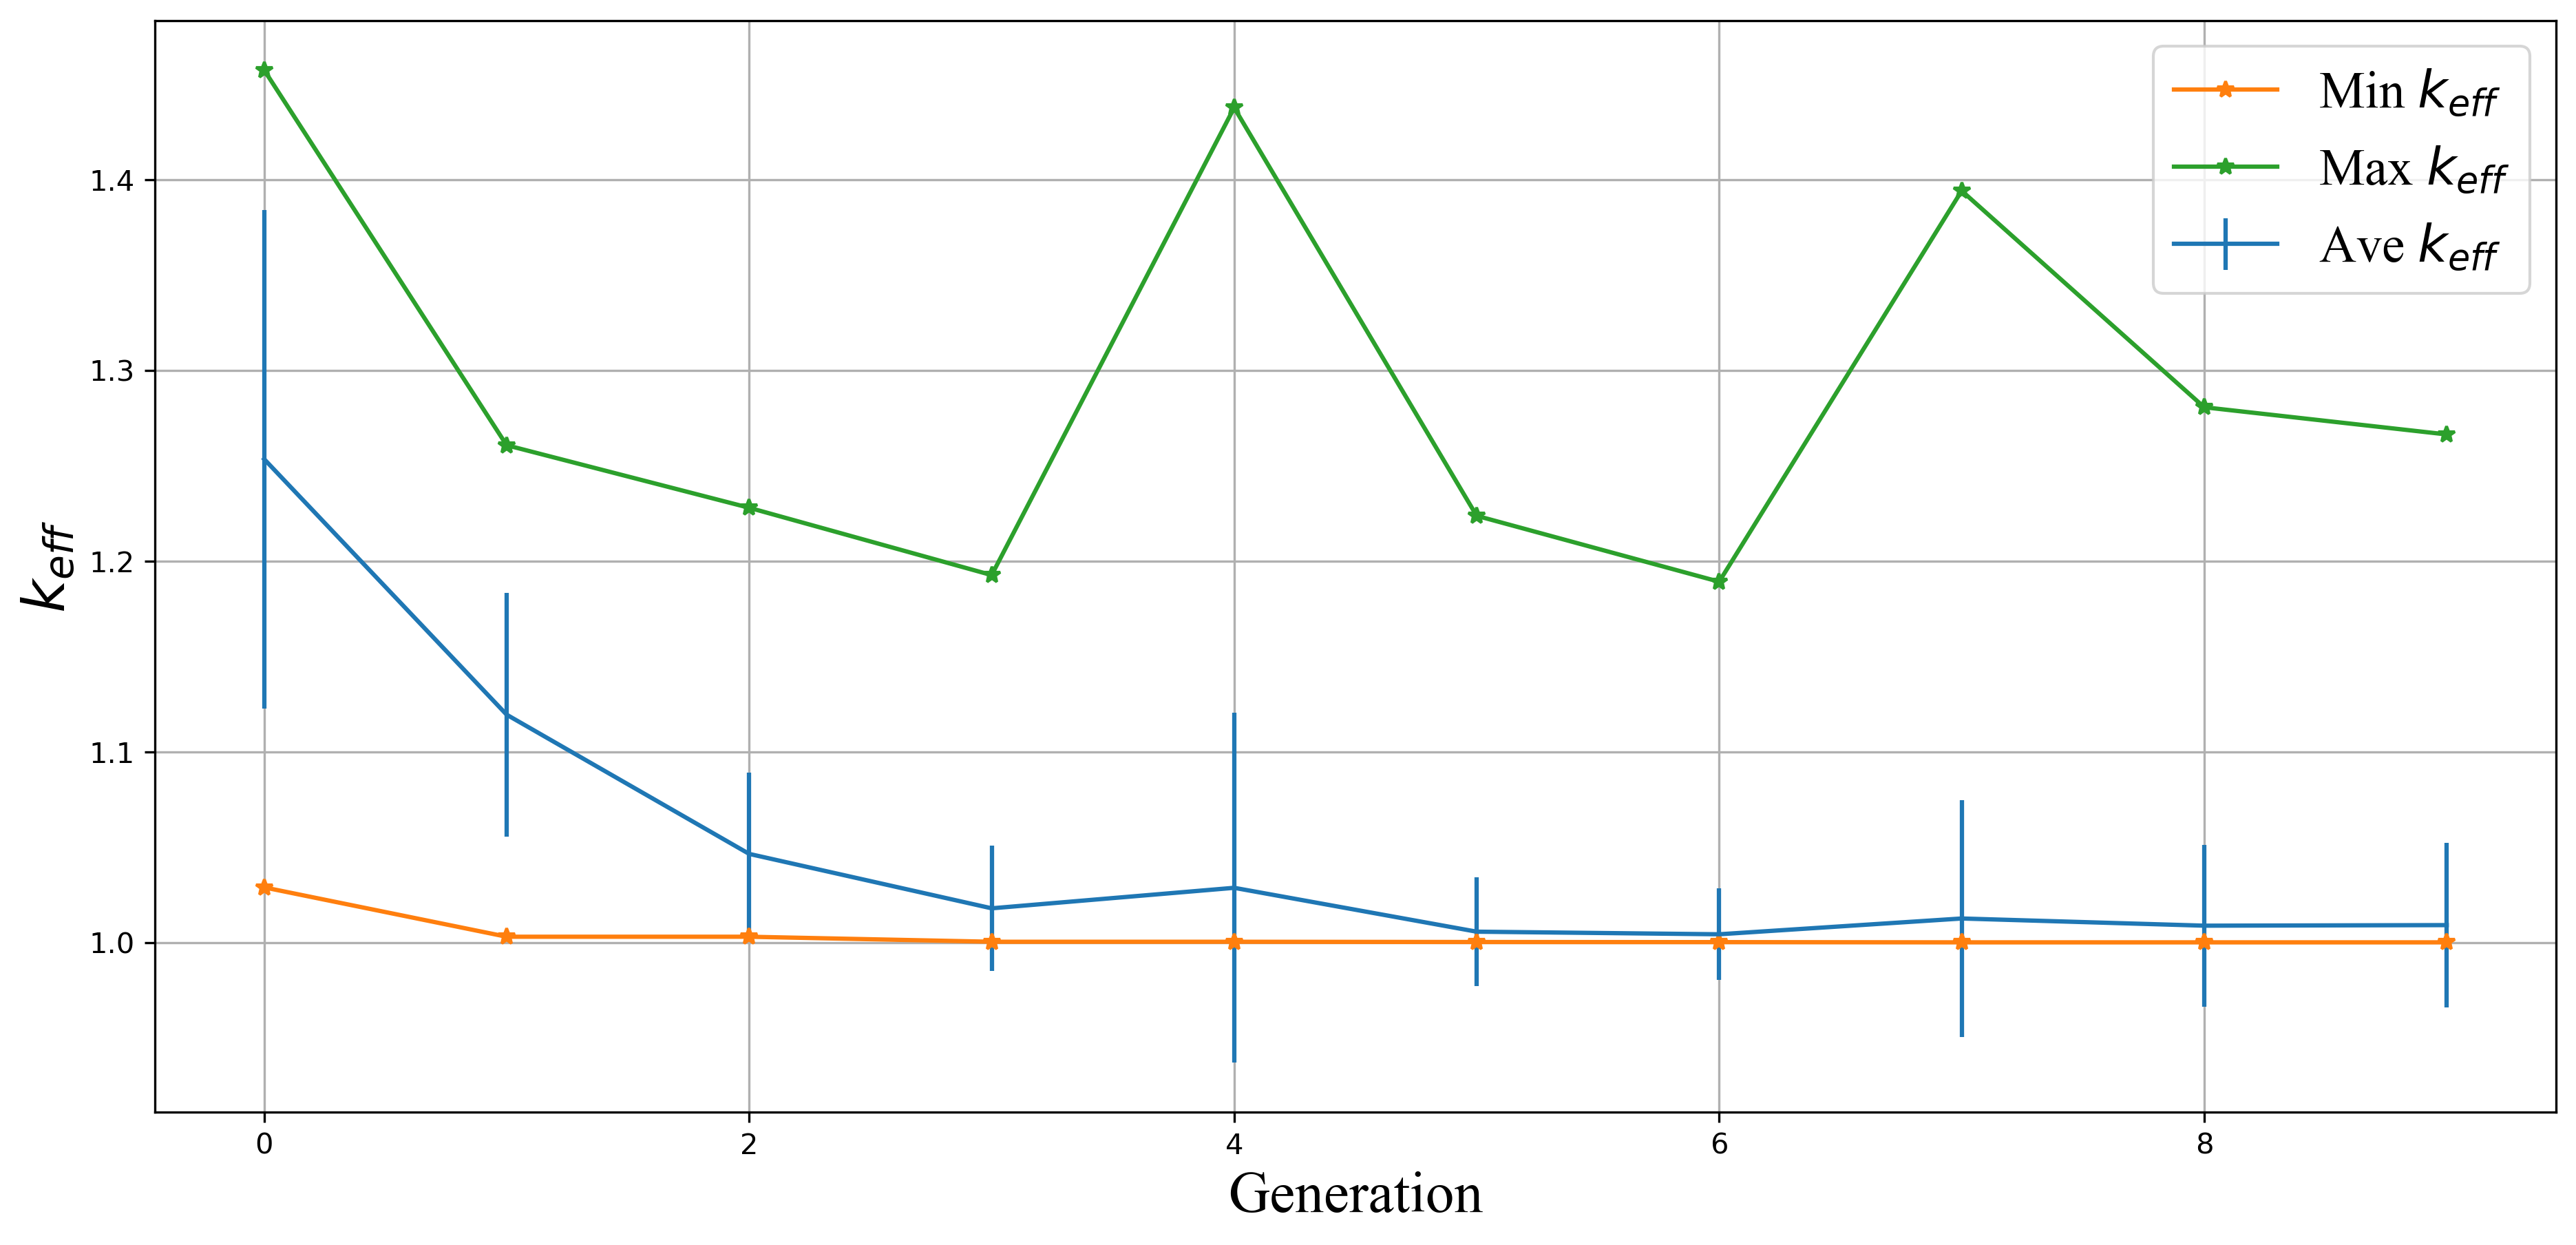
\includegraphics[width=1.1\linewidth]{verification-keff.png}}
        \caption{Minimum, average, and maximum $k_{eff}$ values evolution.}
        \label{fig:verification-keff}
    \end{subfigure}
    \caption{Results for each generation for \gls{ROLLO}'s genetic algorithm optimization 
    to the find the critical radius of a  $^{239}Pu$ bare sphere.}
\end{figure}